


\tikzset{every picture/.style={line width=0.75pt}} %set default line width to 0.75pt        

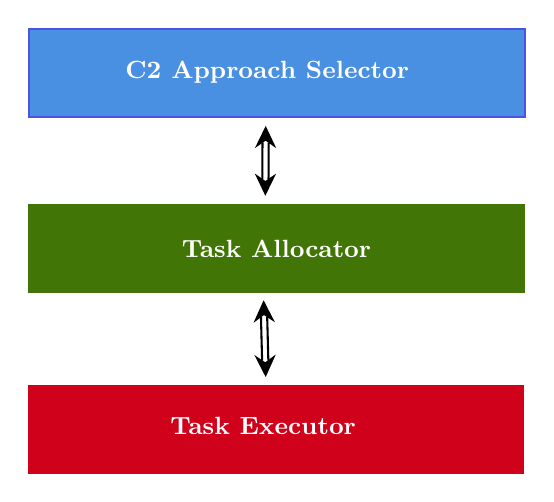
\begin{tikzpicture}[x=0.75pt,y=0.75pt,yscale=-1,xscale=1]
%uncomment if require: \path (0,241); %set diagram left start at 0, and has height of 241

%Flowchart: Process [id:dp48065105856176205] 
\draw  [color={rgb, 255:red, 74; green, 83; blue, 226 }  ,draw opacity=1 ][fill={rgb, 255:red, 74; green, 144; blue, 226 }  ,fill opacity=1 ] (216.5,7.17) -- (455.5,7.17) -- (455.5,49.83) -- (216.5,49.83) -- cycle ;
%Flowchart: Process [id:dp6629894570275567] 
\draw  [color={rgb, 255:red, 65; green, 117; blue, 5 }  ,draw opacity=1 ][fill={rgb, 255:red, 65; green, 117; blue, 5 }  ,fill opacity=1 ] (216.42,92.33) -- (455.08,92.33) -- (455.08,134) -- (216.42,134) -- cycle ;
%Straight Lines [id:da7026427833669057] 
\draw    (331.22,145.96) -- (331.78,166.96)(328.22,146.04) -- (328.78,167.04) ;
\draw [shift={(330.5,175)}, rotate = 268.45] [fill={rgb, 255:red, 0; green, 0; blue, 0 }  ][line width=0.75]  [draw opacity=0] (10.72,-5.15) -- (0,0) -- (10.72,5.15) -- (7.12,0) -- cycle    ;
\draw [shift={(329.5,138)}, rotate = 88.45] [fill={rgb, 255:red, 0; green, 0; blue, 0 }  ][line width=0.75]  [draw opacity=0] (10.72,-5.15) -- (0,0) -- (10.72,5.15) -- (7.12,0) -- cycle    ;
%Flowchart: Process [id:dp18610523674883006] 
\draw  [color={rgb, 255:red, 208; green, 2; blue, 27 }  ,draw opacity=1 ][fill={rgb, 255:red, 208; green, 2; blue, 27 }  ,fill opacity=1 ] (216.33,179.33) -- (454.33,179.33) -- (454.33,221.33) -- (216.33,221.33) -- cycle ;
%Straight Lines [id:da8423233165938356] 
\draw    (331.96,62.01) -- (331.87,79.67)(328.96,61.99) -- (328.87,79.66) ;
\draw [shift={(330.33,87.67)}, rotate = 270.28] [fill={rgb, 255:red, 0; green, 0; blue, 0 }  ][line width=0.75]  [draw opacity=0] (10.72,-5.15) -- (0,0) -- (10.72,5.15) -- (7.12,0) -- cycle    ;
\draw [shift={(330.5,54)}, rotate = 90.28] [fill={rgb, 255:red, 0; green, 0; blue, 0 }  ][line width=0.75]  [draw opacity=0] (10.72,-5.15) -- (0,0) -- (10.72,5.15) -- (7.12,0) -- cycle    ;

% Text Node
\draw (331.25,28) node  [align=left] {\textbf{{\small \textcolor[rgb]{1,1,1}{C2 Approach Selector}}}};
% Text Node
\draw (331.25,113.17) node  [align=left] { \ \ \textbf{{\small \textcolor[rgb]{1,1,1}{ Task Allocator}}}};
% Text Node
\draw (329.25,198.31) node  [align=left] {{\small \textbf{\textcolor[rgb]{1,1,1}{Task Executor}}}};


\end{tikzpicture}